> 本章在第五章方向余弦矩阵的基础上，讨论方向余弦矩阵的时间变化率，从而引入相对转动角速度 $\vec{\omega}_{ij}$ 的概念，并给出科里奥利公式与角速度叠加定理。
\section{固结在动系上的点的相对速度}
设 $i$ 系与 $j$ 系为两个原点重合的右手笛卡尔直角坐标系，其中 $j$ 系相对于 $i$ 系运动（动系）。记 $\boldsymbol{e}_i$、$\boldsymbol{e}_j$ 分别为固定在 $i$ 系、$j$ 系中的单位矢量列阵，$\boldsymbol{A}_{ij}$ 为从 $j$ 系到 $i$ 系的坐标变换矩阵（方向余弦矩阵，见第五章），即
\[
\boldsymbol{e}_i=\boldsymbol{A}_{ij}\boldsymbol{e}_j.
\]
\begin{center}
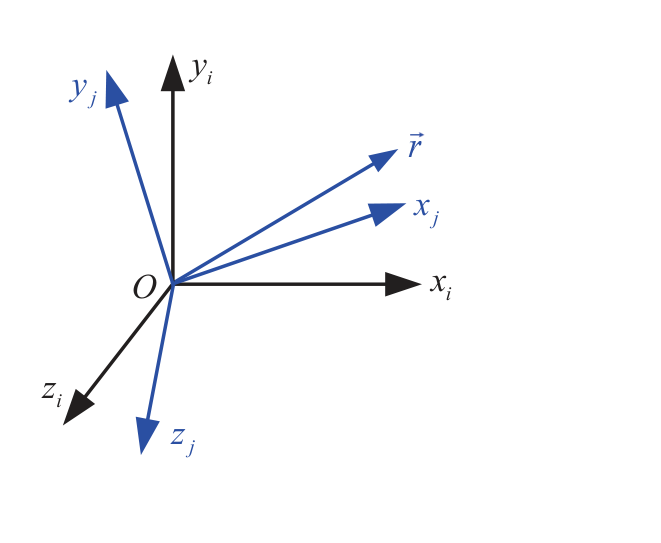
\includegraphics[width=0.80\textwidth]{Figure/SystemDynamicsModelingAndSimulation_63.png}
\par\vspace{0.2em}{\small\kaishu 固结在动系上的点的相对速度示意图}
\end{center}
对于空间任一点 $P$，设其位矢为 $\vec{r}$，在 $i$ 系与 $j$ 系中的坐标列阵分别为 $\boldsymbol{r}_i$ 与 $\boldsymbol{r}_j$，则
\[
\boldsymbol{r}_i=\boldsymbol{A}_{ij}\boldsymbol{r}_j.
\]
若点 $P$ \textbf{固结在动系 $j$ 中}，则 $\boldsymbol{r}_j$ 为常列阵，$\dot{\boldsymbol{r}}_j=\boldsymbol{0}$，于是
\[
\dot{\boldsymbol{r}}_i=\dot{\boldsymbol{A}}_{ij}\boldsymbol{r}_j+\boldsymbol{A}_{ij}\dot{\boldsymbol{r}}_j=\dot{\boldsymbol{A}}_{ij}\boldsymbol{r}_j.
\]
\begin{theorem}[固结在动系上的点的相对速度列阵]
固结在动系 $j$ 中的点，其位矢在定系 $i$ 中的坐标列阵的时间变化率为

\[
\dot{\boldsymbol{r}}_i=\dot{\boldsymbol{A}}_{ij}\boldsymbol{r}_j.
\]
\end{theorem}
\section{两右手笛卡尔直角坐标系的相对方位}
\begin{theorem}[方向余弦矩阵为正交矩阵]
方向余弦矩阵 $\boldsymbol{A}_{ij}$ 的逆等于其转置：

\[
\boldsymbol{A}_{ij}^{-1}=\boldsymbol{A}_{ij}^{\mathrm{T}}
\quad\Longrightarrow\quad
\begin{cases}
\boldsymbol{I}_3=\boldsymbol{A}_{ij}\boldsymbol{A}_{ij}^{\mathrm{T}},\\
\boldsymbol{I}_3=\boldsymbol{A}_{ij}^{\mathrm{T}}\boldsymbol{A}_{ij}.
\end{cases}
\]
\end{theorem}
（坐标系示意同 6.1 节图，原点重合的两组单位矢量基由 $\boldsymbol{A}_{ij}$ 联系。）
\section{方向余弦矩阵的时间变化率（\texorpdfstring{$\boldsymbol{I}_3=\boldsymbol{A}_{ij}\boldsymbol{A}_{ij}^{\mathrm{T}}$}{I_3=AijAijT}）}
\begin{theorem}[$\dot{\boldsymbol{A}}_{ij}$ 的左乘分解]
若 $\boldsymbol{I}_3=\boldsymbol{A}_{ij}\boldsymbol{A}_{ij}^{\mathrm{T}}$，则 $\dot{\boldsymbol{A}}_{ij}\boldsymbol{A}_{ij}^{\mathrm{T}}$ 为反对称矩阵。记

\[
\dot{\boldsymbol{A}}_{ij}\boldsymbol{A}_{ij}^{\mathrm{T}}=:\tilde{\boldsymbol{b}},
\]

则方向余弦矩阵的时间变化率可表示为

\[
\dot{\boldsymbol{A}}_{ij}=\tilde{\boldsymbol{b}}\boldsymbol{A}_{ij}.
\]
\end{theorem}
\begin{proof}[推导]
对 $\boldsymbol{I}_3=\boldsymbol{A}_{ij}\boldsymbol{A}_{ij}^{\mathrm{T}}$ 两端求时间导数：

\[
\boldsymbol{O}_3=\frac{\mathrm{d}}{\mathrm{d}t}\left(\boldsymbol{A}_{ij}\boldsymbol{A}_{ij}^{\mathrm{T}}\right)
=\dot{\boldsymbol{A}}_{ij}\boldsymbol{A}_{ij}^{\mathrm{T}}+\boldsymbol{A}_{ij}\dot{\boldsymbol{A}}_{ij}^{\mathrm{T}}
=\left(\dot{\boldsymbol{A}}_{ij}\boldsymbol{A}_{ij}^{\mathrm{T}}\right)+\left(\dot{\boldsymbol{A}}_{ij}\boldsymbol{A}_{ij}^{\mathrm{T}}\right)^{\mathrm{T}},
\]

其中 $\boldsymbol{O}_3$ 为三阶零矩阵。上式表明 $\dot{\boldsymbol{A}}_{ij}\boldsymbol{A}_{ij}^{\mathrm{T}}$ 与其转置之和为零矩阵，故 $\dot{\boldsymbol{A}}_{ij}\boldsymbol{A}_{ij}^{\mathrm{T}}$ 为反对称矩阵。

令 $\tilde{\boldsymbol{b}}:=\dot{\boldsymbol{A}}_{ij}\boldsymbol{A}_{ij}^{\mathrm{T}}$，将 $\dot{\boldsymbol{A}}_{ij}\boldsymbol{A}_{ij}^{\mathrm{T}}=\tilde{\boldsymbol{b}}$ 两端右乘 $\boldsymbol{A}_{ij}$，并利用 $\boldsymbol{A}_{ij}^{\mathrm{T}}\boldsymbol{A}_{ij}=\boldsymbol{I}_3$，得

\[
\dot{\boldsymbol{A}}_{ij}\boldsymbol{A}_{ij}^{\mathrm{T}}\boldsymbol{A}_{ij}=\tilde{\boldsymbol{b}}\boldsymbol{A}_{ij}
\quad\Longrightarrow\quad
\dot{\boldsymbol{A}}_{ij}=\tilde{\boldsymbol{b}}\boldsymbol{A}_{ij}.
\]
\end{proof}
\section{方向余弦矩阵的时间变化率（\texorpdfstring{$\boldsymbol{I}_3=\boldsymbol{A}_{ij}^{\mathrm{T}}\boldsymbol{A}_{ij}$}{I_3=AijTAij}）}
\begin{theorem}[$\dot{\boldsymbol{A}}_{ij}$ 的右乘分解]
若 $\boldsymbol{I}_3=\boldsymbol{A}_{ij}^{\mathrm{T}}\boldsymbol{A}_{ij}$，则 $\boldsymbol{A}_{ij}^{\mathrm{T}}\dot{\boldsymbol{A}}_{ij}$ 为反对称矩阵。记

\[
\boldsymbol{A}_{ij}^{\mathrm{T}}\dot{\boldsymbol{A}}_{ij}=:\tilde{\boldsymbol{d}},
\]

则方向余弦矩阵的时间变化率可表示为

\[
\dot{\boldsymbol{A}}_{ij}=\boldsymbol{A}_{ij}\tilde{\boldsymbol{d}}.
\]
\end{theorem}
\begin{proof}[推导]
对 $\boldsymbol{I}_3=\boldsymbol{A}_{ij}^{\mathrm{T}}\boldsymbol{A}_{ij}$ 两端求时间导数：

\[
\boldsymbol{O}_3=\frac{\mathrm{d}}{\mathrm{d}t}\left(\boldsymbol{A}_{ij}^{\mathrm{T}}\boldsymbol{A}_{ij}\right)
=\dot{\boldsymbol{A}}_{ij}^{\mathrm{T}}\boldsymbol{A}_{ij}+\boldsymbol{A}_{ij}^{\mathrm{T}}\dot{\boldsymbol{A}}_{ij}
=\left(\boldsymbol{A}_{ij}^{\mathrm{T}}\dot{\boldsymbol{A}}_{ij}\right)^{\mathrm{T}}+\left(\boldsymbol{A}_{ij}^{\mathrm{T}}\dot{\boldsymbol{A}}_{ij}\right),
\]

故 $\boldsymbol{A}_{ij}^{\mathrm{T}}\dot{\boldsymbol{A}}_{ij}$ 为反对称矩阵。

令 $\tilde{\boldsymbol{d}}:=\boldsymbol{A}_{ij}^{\mathrm{T}}\dot{\boldsymbol{A}}_{ij}$，将 $\boldsymbol{A}_{ij}^{\mathrm{T}}\dot{\boldsymbol{A}}_{ij}=\tilde{\boldsymbol{d}}$ 两端左乘 $\boldsymbol{A}_{ij}$，并利用 $\boldsymbol{A}_{ij}\boldsymbol{A}_{ij}^{\mathrm{T}}=\boldsymbol{I}_3$，得

\[
\boldsymbol{A}_{ij}\boldsymbol{A}_{ij}^{\mathrm{T}}\dot{\boldsymbol{A}}_{ij}=\boldsymbol{A}_{ij}\tilde{\boldsymbol{d}}
\quad\Longrightarrow\quad
\dot{\boldsymbol{A}}_{ij}=\boldsymbol{A}_{ij}\tilde{\boldsymbol{d}}.
\]
\end{proof}
\section{方向余弦矩阵的时间变化率（相对转动角速度的引入）}
综合 6.3、6.4 两节，方向余弦矩阵的时间变化率满足
\[
\begin{cases}
\dot{\boldsymbol{A}}_{ij}\boldsymbol{A}_{ij}^{\mathrm{T}}=\tilde{\boldsymbol{b}},\\
\boldsymbol{A}_{ij}^{\mathrm{T}}\dot{\boldsymbol{A}}_{ij}=\tilde{\boldsymbol{d}},
\end{cases}
\quad\Longrightarrow\quad
\begin{cases}
\dot{\boldsymbol{A}}_{ij}=\tilde{\boldsymbol{b}}\boldsymbol{A}_{ij},\\
\dot{\boldsymbol{A}}_{ij}=\boldsymbol{A}_{ij}\tilde{\boldsymbol{d}},
\end{cases}
\quad\Longrightarrow\quad
\tilde{\boldsymbol{b}}\boldsymbol{A}_{ij}=\boldsymbol{A}_{ij}\tilde{\boldsymbol{d}}.
\]
\begin{theorem}[相对转动角速度]
结合方向余弦矩阵的坐标变换性质可知，$\tilde{\boldsymbol{b}}$ 与 $\tilde{\boldsymbol{d}}$ 应为某一个与坐标系 $i$ 和坐标系 $j$ 相对方位有关的矢量在 $i$ 系和 $j$ 系中的投影列阵的叉乘矩阵。该矢量记为 $\vec{\omega}_{ij}$，称为 $j$ 系相对于 $i$ 系的\textbf{相对转动角速度}：

\[
\vec{\omega}_{ij}=\boldsymbol{e}_i^{\mathrm{T}}\boldsymbol{b}=\boldsymbol{e}_j^{\mathrm{T}}\boldsymbol{d}.
\]
\end{theorem}
为便于记忆，作如下变量替换：
\[
\boldsymbol{b}=:\boldsymbol{\omega}_{ij|i},\qquad \boldsymbol{d}=:\boldsymbol{\omega}_{ij|j},
\]
其中 $\boldsymbol{\omega}_{ij|i}$、$\boldsymbol{\omega}_{ij|j}$ 分别为 $\vec{\omega}_{ij}$ 在 $i$ 系、$j$ 系中的投影列阵。
\begin{proof}[说明]
$\tilde{\boldsymbol{b}}\boldsymbol{A}_{ij}=\boldsymbol{A}_{ij}\tilde{\boldsymbol{d}}$ 正是叉乘矩阵在两坐标系间的变换关系（见第五章性质七：$\tilde{\boldsymbol{v}}_{|A}\boldsymbol{A}_{AB}=\boldsymbol{A}_{AB}\tilde{\boldsymbol{v}}_{|B}$），由此可直接看出 $\boldsymbol{b}$ 与 $\boldsymbol{d}$ 是同一矢量在两系中的投影列阵，且满足 $\boldsymbol{b}=\boldsymbol{A}_{ij}\boldsymbol{d}$。
\end{proof}
\section{方向余弦矩阵的时间变化率 \texorpdfstring{$\dot{\boldsymbol{A}}_{ij}$}{Aij}（相对速度）}
采用 $\boldsymbol{\omega}_{ij|i}$、$\boldsymbol{\omega}_{ij|j}$ 记号后，方向余弦矩阵的时间变化率满足
\[
\begin{cases}
\dot{\boldsymbol{A}}_{ij}\boldsymbol{A}_{ij}^{\mathrm{T}}=\tilde{\boldsymbol{\omega}}_{ij|i},\\
\boldsymbol{A}_{ij}^{\mathrm{T}}\dot{\boldsymbol{A}}_{ij}=\tilde{\boldsymbol{\omega}}_{ij|j},
\end{cases}
\quad\Longrightarrow\quad
\begin{cases}
\dot{\boldsymbol{A}}_{ij}=\tilde{\boldsymbol{\omega}}_{ij|i}\boldsymbol{A}_{ij},\\
\dot{\boldsymbol{A}}_{ij}=\boldsymbol{A}_{ij}\tilde{\boldsymbol{\omega}}_{ij|j},
\end{cases}
\quad\Longrightarrow\quad
\begin{cases}
\tilde{\boldsymbol{\omega}}_{ij|i}\boldsymbol{A}_{ij}=\boldsymbol{A}_{ij}\tilde{\boldsymbol{\omega}}_{ij|j},\\
\vec{\omega}_{ij}=\boldsymbol{e}_i^{\mathrm{T}}\tilde{\boldsymbol{\omega}}_{ij|i}=\boldsymbol{e}_j^{\mathrm{T}}\tilde{\boldsymbol{\omega}}_{ij|j}.
\end{cases}
\]
\begin{center}
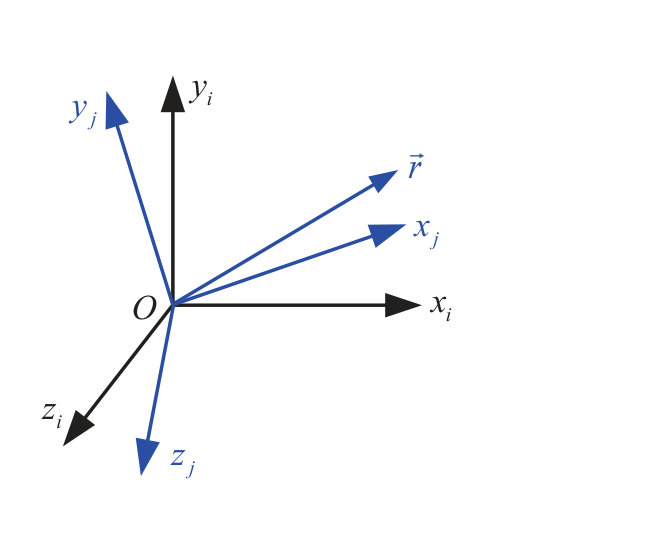
\includegraphics[width=0.80\textwidth]{Figure/SystemDynamicsModelingAndSimulation_65a.png}
\par\vspace{0.2em}{\small\kaishu 固结在动系上的点的相对速度（坐标系示意）}
\end{center}
\textbf{固结在动系上的点的相对速度列阵}：由 6.1 节，结合 $\dot{\boldsymbol{A}}_{ij}=\tilde{\boldsymbol{\omega}}_{ij|i}\boldsymbol{A}_{ij}=\boldsymbol{A}_{ij}\tilde{\boldsymbol{\omega}}_{ij|j}$，得
\[
\dot{\boldsymbol{r}}_i=\dot{\boldsymbol{A}}_{ij}\boldsymbol{r}_j
=\tilde{\boldsymbol{\omega}}_{ij|i}\boldsymbol{A}_{ij}\boldsymbol{r}_j
=\boldsymbol{A}_{ij}\tilde{\boldsymbol{\omega}}_{ij|j}\boldsymbol{r}_j.
\]
\textbf{固结在动系上的点的相对速度矢量}：
\[
\vec{v}\triangleq\boldsymbol{e}_i^{\mathrm{T}}\dot{\boldsymbol{r}}_i=\vec{\omega}_{ij}\times\vec{r}.
\]
\begin{center}
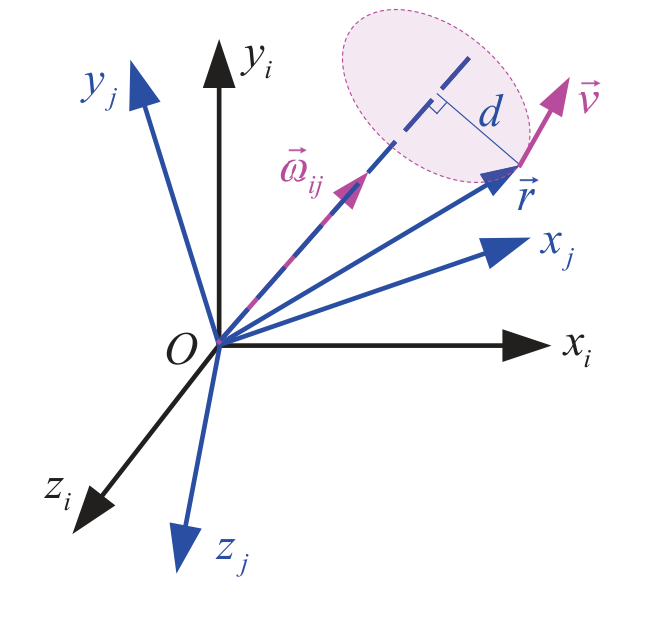
\includegraphics[width=0.80\textwidth]{Figure/SystemDynamicsModelingAndSimulation_65b.png}
\par\vspace{0.2em}{\small\kaishu 相对速度矢量 $\vec{v}$ 与 $\vec{\omega}_{ij}$、$\vec{r}$ 的几何关系}
\end{center}
\begin{theorem}[相对速度的性质]
由 $\vec{v}=\vec{\omega}_{ij}\times\vec{r}$ 可知

\[
\vec{v}\perp\vec{\omega}_{ij},\qquad \vec{v}\perp\vec{r},
\]

\[
|\vec{v}|=|\vec{\omega}_{ij}|\,|\vec{r}|\,\sin\langle\vec{\omega}_{ij},\vec{r}\rangle=|\vec{\omega}_{ij}|\,d,
\]

其中 $d$ 为 $\vec{r}$ 的端点（动点）到 $\vec{\omega}_{ij}$ 轴线的垂直距离。当 $\vec{r}=\alpha\,\vec{\omega}_{ij}$（即动点位于角速度轴上）时，$\vec{v}=\vec{0}$。

由此可知，$j$ 系相对于 $i$ 系作\textbf{瞬时定轴转动}，瞬时转轴沿 $\vec{\omega}_{ij}$ 方向，相对转动角速度为 $\vec{\omega}_{ij}$。
\end{theorem}
\section{科里奥利公式}
\begin{center}
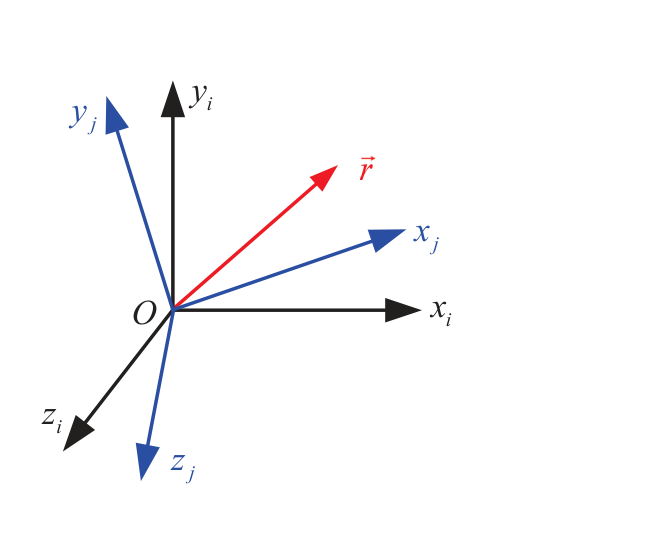
\includegraphics[width=0.80\textwidth]{Figure/SystemDynamicsModelingAndSimulation_66.png}
\par\vspace{0.2em}{\small\kaishu 科里奥利公式推导用坐标系}
\end{center}
设 $\vec{r}$ 为\textbf{任意}矢量（不要求固结于动系），其坐标列阵满足
\[
\vec{r}=\boldsymbol{e}_i^{\mathrm{T}}\boldsymbol{r}_i=\boldsymbol{e}_j^{\mathrm{T}}\boldsymbol{r}_j,\qquad
\boldsymbol{r}_i=\boldsymbol{A}_{ij}\boldsymbol{r}_j.
\]
矢量 $\vec{r}$ 的坐标列阵的时间变化率为
\[
\dot{\boldsymbol{r}}_i=\boldsymbol{A}_{ij}\dot{\boldsymbol{r}}_j+\dot{\boldsymbol{A}}_{ij}\boldsymbol{r}_j
=\boldsymbol{A}_{ij}\dot{\boldsymbol{r}}_j+\boldsymbol{A}_{ij}\tilde{\boldsymbol{\omega}}_{ij|j}\boldsymbol{r}_j.
\]
于是
\[
\boldsymbol{e}_i^{\mathrm{T}}\dot{\boldsymbol{r}}_i
=\boldsymbol{e}_i^{\mathrm{T}}\boldsymbol{A}_{ij}\dot{\boldsymbol{r}}_j
+\boldsymbol{e}_i^{\mathrm{T}}\boldsymbol{A}_{ij}\tilde{\boldsymbol{\omega}}_{ij|j}\boldsymbol{r}_j.
\]
\begin{theorem}[科里奥利公式]
任意矢量 $\vec{r}$ 在 $i$ 系与 $j$ 系中的时间导数满足

\[
\left.\frac{\mathrm{d}\vec{r}}{\mathrm{d}t}\right|_{i}
=\left.\frac{\mathrm{d}\vec{r}}{\mathrm{d}t}\right|_{j}+\vec{\omega}_{ij}\times\vec{r}.
\]
\end{theorem}
\begin{proof}[推导]
由 $\boldsymbol{e}_i=\boldsymbol{A}_{ij}\boldsymbol{e}_j$ 转置并利用 $\boldsymbol{A}_{ij}^{\mathrm{T}}\boldsymbol{A}_{ij}=\boldsymbol{I}_3$，得 $\boldsymbol{e}_i^{\mathrm{T}}\boldsymbol{A}_{ij}=\boldsymbol{e}_j^{\mathrm{T}}$。于是上式中第一项为

\[
\boldsymbol{e}_i^{\mathrm{T}}\boldsymbol{A}_{ij}\dot{\boldsymbol{r}}_j=\boldsymbol{e}_j^{\mathrm{T}}\dot{\boldsymbol{r}}_j=\left.\frac{\mathrm{d}\vec{r}}{\mathrm{d}t}\right|_{j},
\]

第二项为

\[
\boldsymbol{e}_i^{\mathrm{T}}\boldsymbol{A}_{ij}\tilde{\boldsymbol{\omega}}_{ij|j}\boldsymbol{r}_j
=\boldsymbol{e}_j^{\mathrm{T}}\tilde{\boldsymbol{\omega}}_{ij|j}\boldsymbol{r}_j=\vec{\omega}_{ij}\times\vec{r}.
\]

代入即得科里奥利公式。

特别地，当 $\vec{r}$ 固结于 $j$ 系时 $\dot{\boldsymbol{r}}_j=\boldsymbol{0}$，退化为 6.6 节的相对速度公式：

\[
\left.\frac{\mathrm{d}\vec{r}}{\mathrm{d}t}\right|_{i}=\vec{\omega}_{ij}\times\vec{r}.
\]
\end{proof}
\section{角速度叠加定理}
\begin{center}
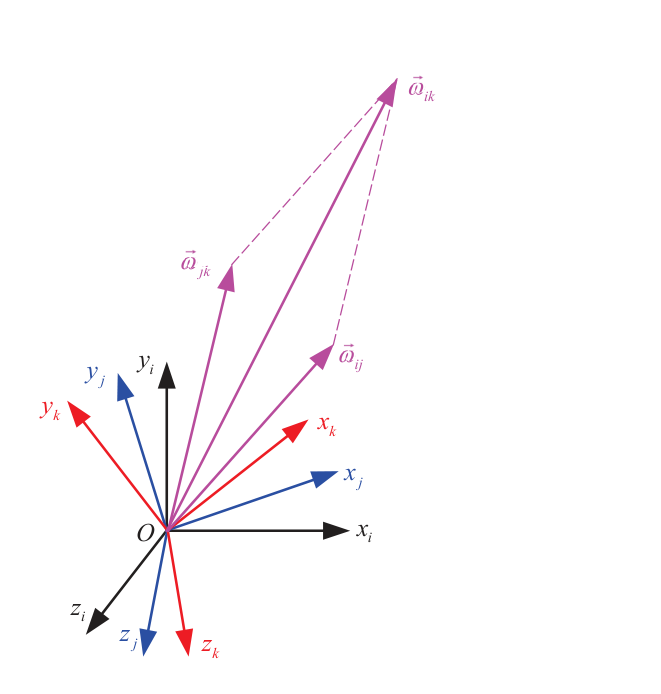
\includegraphics[width=0.55\textwidth]{Figure/SystemDynamicsModelingAndSimulation_67.png}
\par\vspace{0.2em}{\small\kaishu 三个坐标系的相对方位与角速度合成}
\end{center}
考虑三个右手笛卡尔直角坐标系 $i$、$j$、$k$，其相对方位满足
\[
\boldsymbol{e}_i=\boldsymbol{A}_{ij}\boldsymbol{e}_j=\boldsymbol{A}_{ij}\boldsymbol{A}_{jk}\boldsymbol{e}_k,
\]
\[
\boldsymbol{A}_{ik}=\boldsymbol{e}_i\cdot\boldsymbol{e}_k^{\mathrm{T}}=\boldsymbol{A}_{ij}\boldsymbol{A}_{jk},
\]
\[
\dot{\boldsymbol{A}}_{ik}=\dot{\boldsymbol{A}}_{ij}\boldsymbol{A}_{jk}+\boldsymbol{A}_{ij}\dot{\boldsymbol{A}}_{jk}.
\]
将 $\dot{\boldsymbol{A}}_{ik}=\boldsymbol{A}_{ik}\tilde{\boldsymbol{\omega}}_{ik|k}$、$\dot{\boldsymbol{A}}_{ij}=\boldsymbol{A}_{ij}\tilde{\boldsymbol{\omega}}_{ij|j}$、$\dot{\boldsymbol{A}}_{jk}=\boldsymbol{A}_{jk}\tilde{\boldsymbol{\omega}}_{jk|k}$ 代入上式，得
\[
\boldsymbol{A}_{ik}\tilde{\boldsymbol{\omega}}_{ik|k}
=\boldsymbol{A}_{ij}\tilde{\boldsymbol{\omega}}_{ij|j}\boldsymbol{A}_{jk}+\boldsymbol{A}_{ij}\boldsymbol{A}_{jk}\tilde{\boldsymbol{\omega}}_{jk|k}.
\]
\begin{theorem}[角速度叠加定理]
坐标系 $k$ 相对于坐标系 $i$ 的角速度，等于 $j$ 系相对 $i$ 系的角速度与 $k$ 系相对 $j$ 系的角速度之和：

\[
\vec{\omega}_{ik}=\vec{\omega}_{ij}+\vec{\omega}_{jk}.
\]
\end{theorem}
\begin{proof}[推导]
由叉乘矩阵的坐标变换关系（第五章性质七）$\tilde{\boldsymbol{\omega}}_{ij|j}\boldsymbol{A}_{jk}=\boldsymbol{A}_{jk}\tilde{\boldsymbol{\omega}}_{ij|k}$，并利用 $\boldsymbol{A}_{ij}\boldsymbol{A}_{jk}=\boldsymbol{A}_{ik}$，上式可化为

\[
\boldsymbol{A}_{ik}\tilde{\boldsymbol{\omega}}_{ik|k}
=\boldsymbol{A}_{ik}\tilde{\boldsymbol{\omega}}_{ij|k}+\boldsymbol{A}_{ik}\tilde{\boldsymbol{\omega}}_{jk|k},
\]

即

\[
\tilde{\boldsymbol{\omega}}_{ik|k}=\tilde{\boldsymbol{\omega}}_{ij|k}+\tilde{\boldsymbol{\omega}}_{jk|k},
\]

等价地，在 $i$ 系中表示为

\[
\tilde{\boldsymbol{\omega}}_{ik|i}=\tilde{\boldsymbol{\omega}}_{ij|i}+\tilde{\boldsymbol{\omega}}_{jk|i},
\]

即

\[
\boldsymbol{\omega}_{ik|i}=\boldsymbol{\omega}_{ij|i}+\boldsymbol{\omega}_{jk|i}.
\]

由 6.5 节的关系 $\vec{\omega}_{ij}=\boldsymbol{e}_i^{\mathrm{T}}\boldsymbol{\omega}_{ij|i}$，得角速度叠加定理

\[
\vec{\omega}_{ik}=\vec{\omega}_{ij}+\vec{\omega}_{jk}.
\]
\end{proof}
